\chapter{有机化学中的氧化与还原}\label{ch:b1:organic-redox}

一瓶敞口放置的葡萄酒，几天之内便会变成醋：细菌利用空气中的氧，
将乙醇氧化为乙酸。酮与生成它的醇相差两个氢原子——
若恰当地计数，则相差两个电子。有机氧化与还原
看上去不像
\cref{ch:b1:nernst}中金属离子之间的电子交换，
因为电子随质子或氢负离子一起转移，但
记账方式是相同的。本章为碳原子指定氧化级别，
并据此预测每种醇被氧化后得到什么，并
介绍可还原羰基化合物的氢化试剂，同时
关注每种试剂不影响哪些基团。

\begin{recall}
氧化数、半反应式及氧化还原方程式的配平见
\cref{ch:b1:nernst}；醇和碳原子的分类见
\cref{ch:b1:electronic-effects}；缩醛及羰基的保护见
\cref{ch:b1:acetals-protection}；格氏加成见
\cref{ch:b1:organomagnesium}。
\end{recall}

\begin{omfigure}
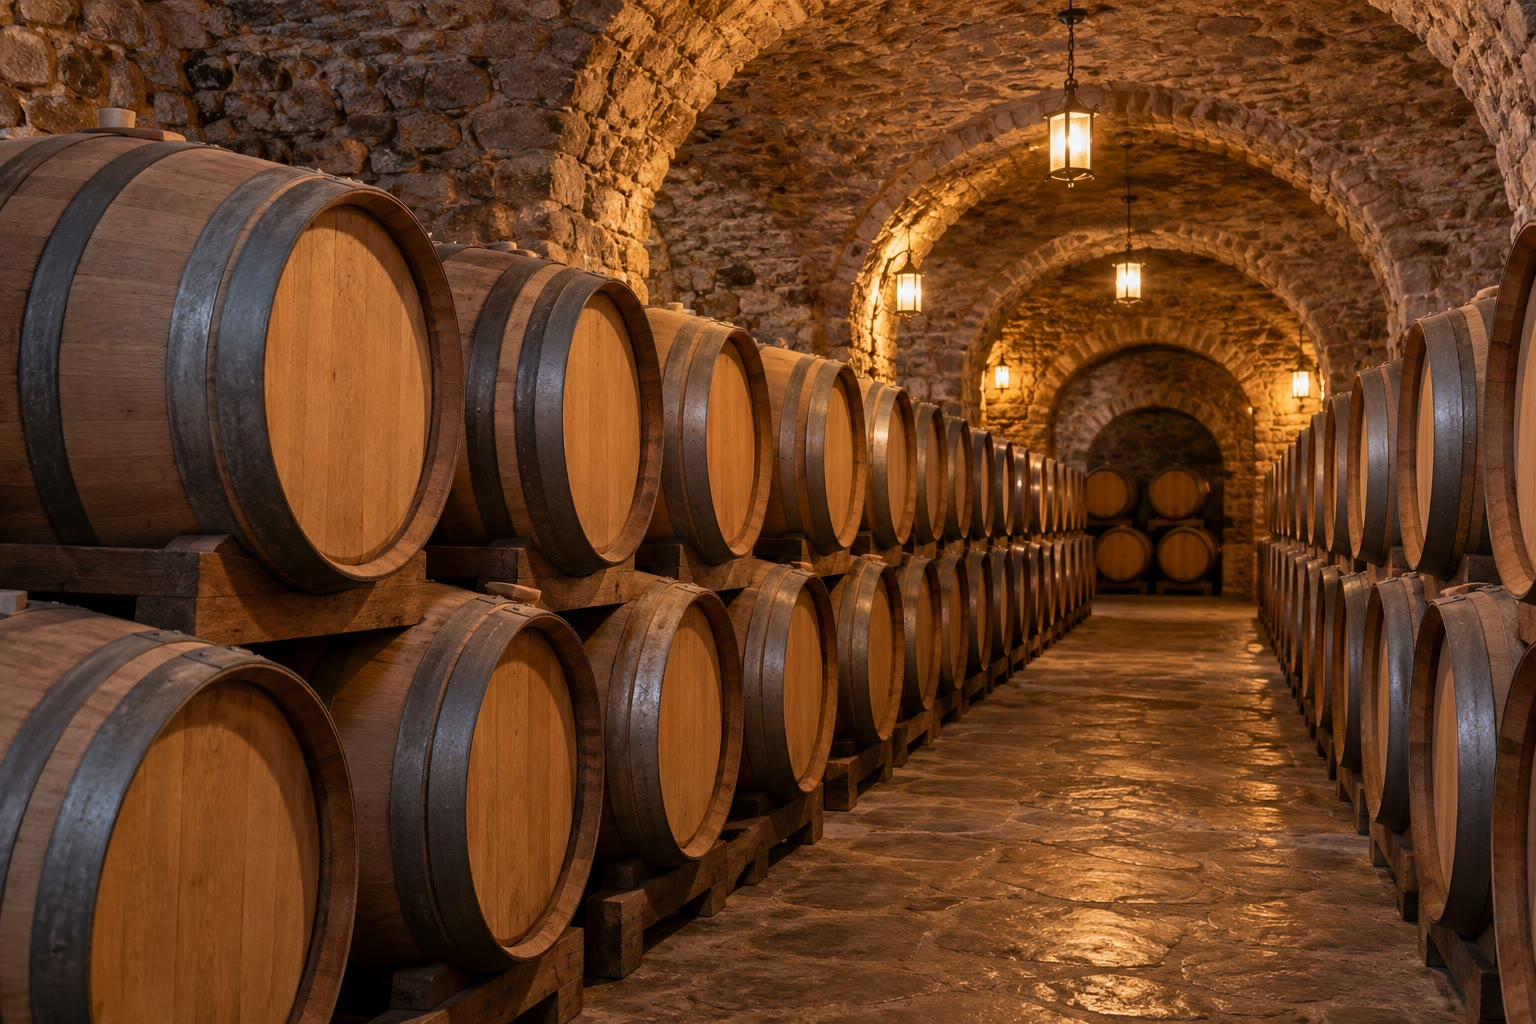
\includegraphics[width=0.58\linewidth]{images/book2/ai/b1-24-wine-cellar.jpg}

{\small 酒窖中陈化的葡萄酒。隔绝空气时，葡萄酒保留其乙醇；
暴露于空气中时，醋酸菌将其氧化为乙酸。}
\end{omfigure}

\section{碳的氧化级别}

\begin{definition}[氧化级别]\label{def:b1:organic-redox:oxidation-level}
碳原子的\emph{氧化级别}\index{氧化级别}是指
氧化数，按
\cref{prop:b1:nernst:on-rules}中的规则求得：每一个与电负性更大的原子
（O、N、卤素）计 $+1$，与氢成的键计 $-1$，与
另一碳原子成的键计 0（双键计两次）。
\end{definition}

\begin{proposition}[碳的氧化数]\label{prop:b1:organic-redox:on-of-carbon}
碳原子的氧化数等于（与 O、N 或卤素成键的数目）
减去（与 H 成键的数目）。在碳骨架相同的
一族化合物中，醇 $\to$ 醛或酮 $\to$
羧酸 $\to$ 二氧化碳，每一步都是转移两个电子的
氧化过程。
\end{proposition}

\begin{proof}
断开每一个键，并将两个电子都给予电负性较大的
伙伴原子：与 H 成键时（H 的电负性小于 C），碳获得一个电子，
每个 C--H 键带 $-1$ 电荷；与 O、N、卤素（电负性更大）成键时，碳失去
一个电子，每个键 $+1$；C--C 键平分电子。由 \ce{-CH2OH}
（与一个碳原子相连的碳为 $-1$）到 \ce{-CHO}（$+1$），再到
\ce{-COOH}（$+3$），每一步氧化数升高 2，即两个电子。
\end{proof}

\begin{omfigure}
\begin{tikzpicture}[font=\small, >={Stealth}]
  \foreach \x/\f/\n in {0/\ce{CH4}/-4, 2.4/\ce{CH3OH}/-2, 4.8/\ce{HCHO}/0, 7.2/\ce{HCOOH}/+2, 9.6/\ce{CO2}/+4} {
    \node[draw, rounded corners, minimum width=1.5cm] at (\x,0) {\f};
    \node[below] at (\x,-0.5) {$\n$};
  }
  \foreach \x in {0.8,3.2,5.6,8.0} \draw[->, thick, omThm] (\x,0) -- ++(0.8,0);
  \node[omThm, above] at (4.8,0.5) {氧化：每步 $-2\,\mathrm{e^-}$（及 $-2\,\ce{H+}$）};
  \node[left] at (-0.9,-0.75) {碳的氧化数：};
\end{tikzpicture}

{\small 一碳族化合物的氧化级别：甲烷、甲醇、
甲醛、甲酸、二氧化碳。每个箭头均为两电子
氧化；逆向看即为还原。}
\end{omfigure}

\begin{method}[有机半反应式的配平]\label{met:b1:organic-redox:balance-organic-redox}
\begin{enumerate}
  \item 写出骨架相同的有机氧化剂与还原剂。
  \item 由发生改变的碳原子的氧化数变化计算电子数
        （或简便地：每失去一对 H 或每得到一个 O，
        计两个电子）。
  \item 用水配平氧，用 \ce{H+} 配平氢，用
        电子配平电荷。
\end{enumerate}
乙醇变为乙酸：\ce{CH3CH2OH + H2O -> CH3COOH + 4H+ + 4e-}。
用酸化的重铬酸盐（\ce{Cr2O7^2- + 14H+ + 6e- -> 2Cr^3+ + 7H2O}），
三个乙醇分子对两个重铬酸根离子：
\ce{3CH3CH2OH + 2Cr2O7^2- + 16H+ -> 3CH3COOH + 4Cr^3+ + 11H2O}.
\end{method}

\section{醇的氧化}

\begin{proposition}[醇被氧化后的产物]\label{prop:b1:organic-redox:alcohol-oxidation}
伯醇 \ce{RCH2OH} 被氧化为醛 \ce{RCHO}，随后
（在水中，与强氧化剂作用）进一步氧化为羧酸 \ce{RCOOH}；
仲醇 \ce{R2CHOH} 氧化为酮 \ce{R2CO}，该酮不再被进一步氧化；
叔醇 \ce{R3COH} 不能被氧化，除非
断裂 C--C 键。
\end{proposition}

\begin{proof}
醇的氧化移去羟基上的氢及
羟基碳上的一个氢，生成 C=O。叔醇的羟基碳
上没有这样的氢。醛的羰基碳上仍连有一个 H，在
水中部分水合为 \ce{RCH(OH)2}，再以同样方式被氧化为
\ce{RCOOH}。酮的该碳上无 H，反应即止。
\end{proof}

在水溶液中，强氧化剂——酸化的重铬酸钾或
高锰酸钾——可将伯醇氧化为酸。若要停在
醛阶段，则随生成随蒸出（醛的沸点低于
由其制得的醇，因醛无 O--H 氢键），或改用
较温和的无水试剂，这些在本科二年级分册中介绍。

\begin{safety}{\ghs[5mm]{GHS03}\,\ghs[5mm]{GHS05}\,\ghs[5mm]{GHS06}\,\ghs[5mm]{GHS07}\,\ghs[5mm]{GHS08}\,\ghs[5mm]{GHS09}}
重铬酸钾是经典的醇类橙色氧化剂，
被列为可能致癌的物质之一：使用时须
仅取少量，并戴手套和护目镜，其含铬废料
须单独收集；如有可能，应优先
选用危害较小的氧化剂。
% ledger: ghs:K2Cr2O7
\end{safety}

\section{用氢化物还原羰基化合物}

\begin{definition}[氢负离子供体]\label{def:b1:organic-redox:hydride-donor}
称\emph{氢负离子供体}\index{氢负离子供体}为可将带成键电子对的氢原子
（\ce{H-}）转移给亲电碳原子的物质。硼氢化钠
\ce{NaBH4} 和氢化铝锂 \ce{LiAlH4} 都是\emph{金属复氢化物}\index{金属复氢化物}
：氢负离子由 \ce{BH4-} 或 \ce{AlH4-} 离子提供，
而非游离离子。
\end{definition}

\begin{omfigure}
\setchemfig{atom sep=2.1em}
\schemestart
\chemfig{H_3B^{-}-[@{bh}]@{h}H}
\+
\chemfig{@{c}C(-[:150]R)(-[:210]R')=[@{co}]@{o}O}
\arrow{->}
\chemfig{C(-[:150]R)(-[:210]R')(-[2]H)-O^{-}}
\arrow{->[\ce{H2O}]}
\chemfig{C(-[:150]R)(-[:210]R')(-[2]H)-OH}
\schemestop
\chemmove{\draw[->, thick, shorten <=2pt, shorten >=3pt](bh) .. controls +(80:9mm) and +(180:7mm) .. (c);
          \draw[->, thick, shorten <=2pt, shorten >=2pt](co) .. controls +(90:6mm) and +(90:6mm) .. (o);}
\par\vspace{6pt}

{\small 硼氢化物还原酮：一对 B--H 成键电子形成新的 C--H
键，同时 C=O 的 $\pi$ 电子对转到氧原子上；醇盐
被溶剂（水或醇）质子化，或于后处理时完成。每个 \ce{BH4-}
可依次提供其四个氢原子。}
\end{omfigure}

\begin{proposition}[两种氢化物的适用范围]\label{prop:b1:organic-redox:hydride-scope}
硼氢化钠用于水或醇中，可将醛还原为
伯醇，将酮还原为仲醇，而对酯、
羧酸、酰胺及 C=C 双键不起作用。氢化铝锂
用于无水乙醚中，还可将酯和羧酸
还原为伯醇，并与水剧烈反应。
\end{proposition}

\begin{proof}
Al--H 键的极性比 B--H 键更强（铝的电负性
小于硼），因此 \ce{AlH4-} 是强得多的氢负离子供体，
能够进攻亲电性较弱的酯羰基和
羧酸根的羰基；同样的反应活性使其能与任何酸性
氢（包括水中的氢）反应。\ce{BH4-} 与水和醇
仅缓慢反应，只进攻亲电性最强的羰基。孤立的
C=C 双键不具亲电性，两者均不能将其还原。
\end{proof}

\section{选择性}

\begin{definition}[化学选择性反应]\label{def:b1:organic-redox:chemoselective}
\emph{化学选择性反应}\index{化学选择性反应}是指
在分子中其他也可能与另一试剂反应的官能团存在下，
仅作用于某一官能团的反应。
\end{definition}

\begin{omfigure}
\begin{tabular}{lcc}
\hline
官能团 & \ce{NaBH4}（醇溶剂） & \ce{LiAlH4}（无水乙醚） \\
\hline
醛 \ce{RCHO} & 伯醇 & 伯醇 \\
酮 \ce{R2CO} & 仲醇 & 仲醇 \\
酯 \ce{RCOOR} & 不反应 & 两种醇 \\
羧酸 \ce{RCOOH} & 不反应（生成盐） & 伯醇 \\
烯烃 \ce{C=C} & 不反应 & 不反应 \\
缩醛 & 不反应 & 不反应 \\
\hline
\end{tabular}

\smallskip
{\small 两种氢化物能还原的物质。硼氢化钠是
化学选择性试剂；氢化铝锂则是作用更强的试剂。}
\end{omfigure}

\begin{example}[一种酮酯]\label{ex:b1:organic-redox:ketoester}
4-氧代戊酸乙酯 \ce{CH3CO(CH2)2COOEt}，与硼氢化钠
反应生成 4-羟基戊酸乙酯：只有酮被还原。与氢化铝锂
反应时两个基团均被还原，得到戊烷-1,4-二醇
（并生成乙醇）。若只还原酯基，则须先将酮保护为
缩醛（见\cref{ch:b1:acetals-protection}）。
\end{example}

\begin{inthelab}[还原酮]
将硼氢化钠分小份加入酮的冷
乙醇溶液中：反应放热，并因试剂与溶剂缓慢反应而冒出氢气。
搅拌后，用稀酸分解过量试剂
（会生成更多氢气，附近不得有明火），然后萃取出醇。
氢化铝锂则不同，仅用于无水乙醚中，
并在惰性气体保护下使用，
其过量部分须极为小心地分解。
\end{inthelab}

\section{练习}

\begin{exercise}[$\star$]\label{exo:b1:organic-redox:1}
求下列化合物中每个碳原子的氧化数：乙醇、乙醛、
乙酸、丙酮和甲酸。
\end{exercise}

\begin{exercise}[$\star$]\label{exo:b1:organic-redox:2}
酸化的重铬酸根与丙-1-醇、丙-2-醇及
2-甲基丙-2-醇分别反应，各得到什么？
\end{exercise}

\begin{exercise}[$\star$]\label{exo:b1:organic-redox:3}
写出酸性条件下丙酮/丙-2-醇与
乙醛/乙醇两个电对的半反应式。
\end{exercise}

\begin{exercise}[$\star$]\label{exo:b1:organic-redox:4}
硼氢化钠与氢化铝锂分别与
丁醛、丁酮、丁酸乙酯和丁酸反应，各得到什么？
\end{exercise}

\begin{exercise}[$\star\star$]\label{exo:b1:organic-redox:5}
配平酸性条件下高锰酸根（\ce{MnO4-}/\ce{Mn^2+}）氧化丙-2-醇的反应，
并计算氧化 \qty{1.20}{g} 醇（$M = \qty{60.0}{g/mol}$）所需
浓度为 \qty{0.020}{mol/L} 的高锰酸根溶液的体积。
\end{exercise}

\begin{exercise}[$\star\star$]\label{exo:b1:organic-redox:6}
如何由丙-1-醇制得丙醛，并使其不再被进一步氧化？
利用沸点数据：丙-1-醇 \qty{97}{\celsius}，丙醛
\qty{48}{\celsius}。
% ledger: bp:propanal, bp:propan-1-ol
\end{exercise}

\begin{exercise}[$\star\star$]\label{exo:b1:organic-redox:7}
写出乙醛在乙醇中被 \ce{BH4-} 还原的反应机理。
产物中哪个原子来自试剂？
\end{exercise}

\begin{exercise}[$\star\star$]\label{exo:b1:organic-redox:8}
用 \ce{NaBH4} 还原丁-2-酮得到手性醇。该醇
是否具有旋光性？为什么？
\end{exercise}

\begin{exercise}[$\star\star$]\label{exo:b1:organic-redox:9}
警方曾用于酒精呼气检测的装置中，橙色的重铬酸根
与乙醇反应后变为绿色。写出该反应，并解释
颜色变化。
\end{exercise}

\begin{exercise}[$\star\star\star$]\label{exo:b1:organic-redox:10}
设计下列化合物的合成路线：2-甲基丁-2-醇可由乙醛与格氏试剂
反应，经氧化后再进行第二次格氏反应得到；戊-3-醇可由丙醛
制得。统计其中氧化与还原步骤的数目。
\end{exercise}

\begin{exercise}[$\star\star\star$]\label{exo:b1:organic-redox:11}
仅还原 4-氧代戊酸甲酯中的酯基，
\ce{CH3CO(CH2)2COOCH3}。借助保护基规划三步反应，
并给出产物。
\end{exercise}

\begin{exercise}[$\star\star\star$]\label{exo:b1:organic-redox:12}
证明在伯醇氧化为羧酸的过程中，
由氧化数及半反应式可知，有四个电子转移。
将此推广至甲烷氧化为二氧化碳的情形。
\end{exercise}

\section{问题：由环己醇到己二酸}

\begin{problem}[{周末问题——环己醇、环己酮与己二酸的氧化级别，
硝酸氧化及其电子转移，
过氧化氢路线，以及每吨己二酸释放的
一氧化二氮质量}]
\label{pb:b1:organic-redox:1}
己二酸（己烷二酸）\ce{HOOC(CH2)4COOH} 大规模生产，
主要用于制造尼龙，多通过硝酸氧化环己醇（并伴有环己酮）制得，
该过程释放出一氧化二氮 \ce{N2O}，它是一种强效
温室气体。摩尔质量（\unit{g/mol}）：\ce{C6H12O} 100.0，
\ce{C6H10O} 98.0，\ce{C6H10O4} 146.0，\ce{N2O} 44.0，\ce{HNO3} 63.0，
\ce{H2O2} 34.0。

\medskip
\noindent\textbf{第一部分——氧化级别。}
\begin{enumerate}
  \item 求环己醇中每个碳原子的氧化数。
  \item 求环己酮中每个碳原子的氧化数。
  \item 求己二酸中每个碳原子的氧化数。
  \item 由环己醇转化为己二酸的过程中，哪些碳原子被氧化，
        断裂的是哪一个键？
  \item 一个环己醇分子失去多少个电子？
  \item 作为酮的环己酮，为何在此过程中仍会被进一步氧化？
\end{enumerate}

\medskip
\noindent\textbf{第二部分——硝酸路线。}
\begin{enumerate}[resume]
  \item 写出酸性条件下由环己醇转化为己二酸的半反应式。
  \item 求 \ce{HNO3} 与 \ce{N2O} 中 N 的氧化数。
  \item 写出 \ce{HNO3}/\ce{N2O} 的半反应式。
  \item 将两个半反应合并，并验证可得
        \ce{C6H12O + 2HNO3 -> C6H10O4 + N2O + 2H2O}。
  \item 每摩尔己二酸所交换的电子的物质的量为
        多少摩尔？
  \item 计算每吨己二酸所消耗的硝酸质量。
\end{enumerate}

\medskip
\noindent\textbf{第三部分——过氧化氢路线。}
\begin{enumerate}[resume]
  \item 写出 \ce{H2O2}/\ce{H2O} 的半反应式。
  \item 写出并配平过氧化氢将环己醇氧化为
        己二酸的反应。
  \item 计算每吨己二酸所需 \ce{H2O2} 的质量。
  \item 唯一的副产物是什么？为何称该路线更为绿色？
  \item 过氧化氢须借助催化剂才能活化。
        利用\cref{exo:b1:nernst:12}，解释为何热力学上有利的
        氧化反应仍可能需要催化剂。
  \item 硼氢化钠与环己酮作用会得到什么？
        写出该反应。
\end{enumerate}

\medskip
\noindent\textbf{第四部分——质量与温室气体。}
\begin{enumerate}[resume]
  \item 计算一吨己二酸中所含的物质的量。
  \item 计算按硝酸路线与之同时生成的 \ce{N2O} 的物质的量。
  \item 按 \qty{95}{\percent} 产率计算，
        每吨己二酸所需环己醇的质量。
  \item 按硝酸路线，每吨己二酸所释放的 \ce{N2O} 质量，
        以吨为单位给出。
\end{enumerate}
\end{problem}
